\section{Holistic parametric approach (1 page)}
\label{section:contribution_1}

Our approach is based on emergent property estimation techniques \cite{hackenberg2012towards} and uses a model-based approach for validating requirements in early phases of development proposed in \cite{hackenberg2014rapid}, relying on partial system models to ease modeling effort. An adaption to the ITS domain of this modeling technique was proposed in \cite{ascher2014early}, facilitating the formulation of multi-objective traffic flows as an optimal control problem consisting of state variables, control variables, constraints and objectives. The approach employs a generic solver for system behavior estimation, which utilizes stochastic optimization techniques.

\begin{figure}[h]
	\centering
	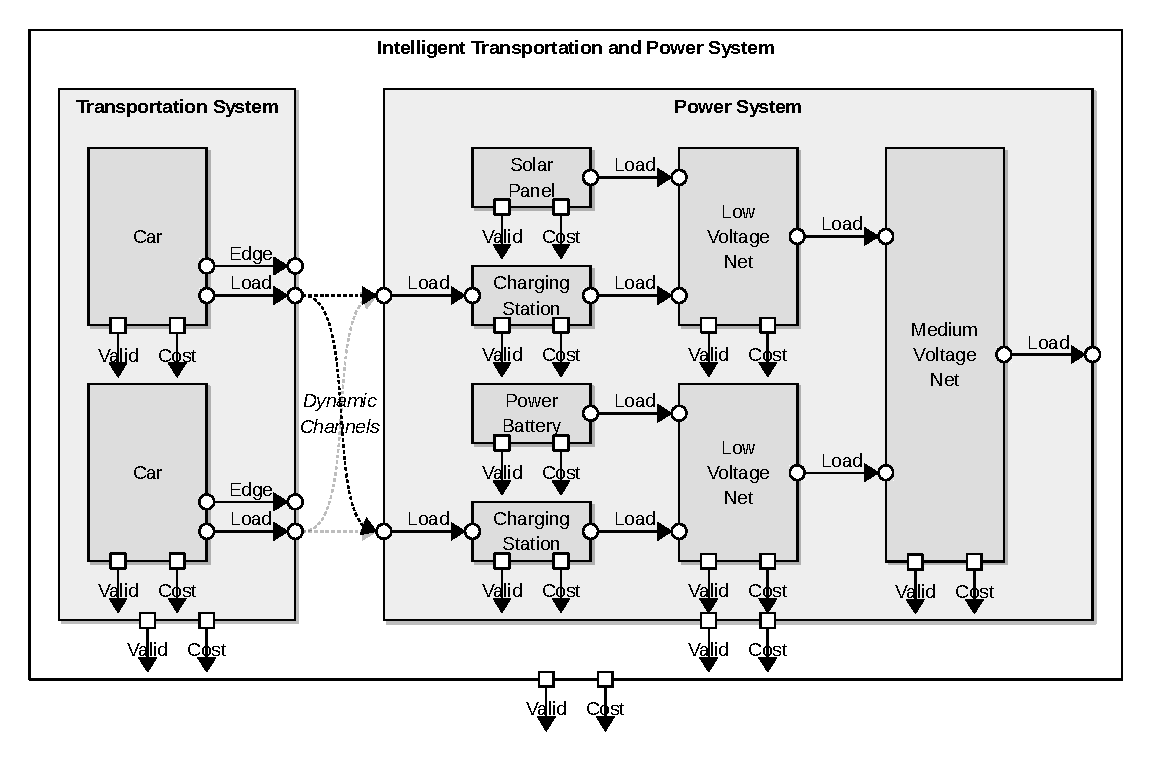
\includegraphics[width=\columnwidth]{../gfx/model.pdf}
	\caption{Overview of the multi-domain system modeling approach including the transportation system and the electricity network.}
	\label{fig:model}
\end{figure}

Model definition is aided by a composite model architecture fitted to transportation scenario modeling seen in Figure~\ref{fig:model}. On it's highest level, the model architecture is represented by the system model, which contains separate models for the traffic and the power system. The traffic model represents the traffic system, in which individual cars within the traffic infrastructure are contained. Similarly, the power model represents the power system, which is comprised by different energy producing or energy consuming power devices, such as solar panels, energy storages and charging stations. Furthermore, the power system includes the electricity infrastructure, such as low-voltage nets and medium-voltage nets. Model components have a set of input and output ports, which represent observations about specific state variables. Directed connections between ports allow the modeling of interactivity between different components.

Subsequently we describe the different components of the model architecture based on their state variables, control variables, constraints and objectives. 

\subsection{Intelligent Transportation and Power System}

\begin{itemize}
	\item Parameter
	\item Interface
	\item Structure
	\item Behavior
\end{itemize}

\subsection{Transportation System}

The traffic model represents the traffic system, in which individual cars within the traffic infrastructure are contained.

\begin{itemize}
	\item Parameter
	\item Interface
	\item Structure
	\item Behavior
\end{itemize}

\subsection{Car}

\begin{itemize}
	\item Parameter
	\item Interface
	\item Structure
	\item Behavior
\end{itemize}

\subsection{Electric Network}

The power model represents the power system, which is comprised by different energy producing or energy consuming power devices, such as solar panels, energy storages and charging stations. Furthermore, the power system includes the electricity infrastructure, such as low-voltage nets and medium-voltage nets.

\begin{itemize}
	\item Parameter
	\item Interface
	\item Structure
	\item Behavior
\end{itemize}

\subsection{Low/Medium Voltage Net}

\begin{itemize}
	\item Parameter
	\item Interface
	\item Structure
	\item Behavior
\end{itemize}

\subsection{Charging Station}

\begin{itemize}
	\item Parameter
	\item Interface
	\item Structure
	\item Behavior
\end{itemize}

\subsection{Power Battery}

\begin{itemize}
	\item Parameter
	\item Interface
	\item Structure
	\item Behavior
\end{itemize}

\subsection{Solar Panel}

\begin{itemize}
	\item Parameter
	\item Interface
	\item Structure
	\item Behavior
\end{itemize}